\documentclass[11pt,a4paper]{article}

\usepackage[
	a4paper,
	left=0.6in,
	right=0.6in,
	top=0.4in,
	bottom=0.4in
]{geometry}
\usepackage{pdfpages}
\usepackage{titlesec}
\titleformat{\section}
	{\normalfont\Large\bfseries}
	{\thesection}{1em}{}
	[\hfill\leaders\hrule\hfill]  % This adds the line on the same line
\usepackage{enumitem}
\usepackage{hyperref}
\usepackage{xcolor}
\usepackage{fontspec}
\setmainfont{Inter}[
	UprightFont = *-Regular,
	% BoldFont = *-SemiBold,
	BoldFont = *-Bold,
	ItalicFont = *-Italic,
	BoldItalicFont = *-SemiBoldItalic
]
\usepackage{fontawesome5}
\usepackage{parskip}
\usepackage{tabularx}

\renewcommand{\normalsize}{\fontsize{10}{14}\selectfont}

% \definecolor{mediumgray}{gray}{0.4} % 0 = black, 1 = white
\definecolor{lighttext}{gray}{0.2} % 0 = black, 1 = white
\definecolor{blue}{HTML}{262f99}

\newcommand{\thinname}{\fontspec{Inter Light}}
\newcommand{\extralight}{\fontspec{Inter ExtraLight}}
\newcommand{\spaced}[2]{%
	{\fontsize{#1}{24}\selectfont\addfontfeature{LetterSpace=10}#2}%
}

\hypersetup{
		colorlinks=true,
		urlcolor=lighttext,
}

% \setlist[itemize]{noitemsep, topsep=2pt}
\setlist[itemize]{noitemsep, topsep=2pt, leftmargin=10pt, font={\fontsize{9}{14}\thinname\selectfont}}

\titleformat{\section}
	{\large\bfseries}
	{}
	{0em}
	{}

\begin{document}
\color{lighttext}

%--------------------
% Header
%--------------------

\begin{center}
{\fontsize{30}{0}\selectfont {\extralight\color{blue} Mateo} \textbf{Torres}}\\
\vspace{0.5em}
\color{blue}
\spaced{8}{I}\spaced{6}{NGENIERO DE}
\spaced{8}{S}\spaced{6}{ISTEMAS \textbf{·}}
\spaced{8}{D}\spaced{6}{ESARROLLADOR}
\end{center}

\vspace{-0.5em}

\begin{center}
{\fontsize{8.5}{0}\selectfont
\addfontfeature{LetterSpace=1.5}
\faEnvelope\ \href{mailto:mateotorresvara@gmail.com}{mateotorresvara@gmail.com} \quad
\faHome\ \href{https://mateotorres.com}{mateotorres.com} \quad
\faGithub\ \href{https://github.com/MateoTVara}{mateotorres}
}
\end{center}

%--------------------
{\color{blue}\fontsize{14.5}{18}\bfseries\selectfont Resumen Profesional} \hfill \rule{0.68\linewidth}{1.2pt}

Estudiante de Ingeniería de Sistemas y técnico en Desarrollo de Sistemas de Información, orientado al detalle,
con enfoque en desarrollo web y un fuerte interés en ciencias de la computación. Experiencia en la creación
de sitios web frontend para pequeños negocios y en el despliegue de soluciones prácticas, con sólidos
conocimientos prácticos en sistemas Linux, particularmente en entornos Arch y basados en Nix. Habilidad
para desarrollar aplicaciones web mantenibles y centradas en el usuario, ampliando continuamente mi
experiencia en programación, ecosistemas Linux y flujos de trabajo modernos de desarrollo. Apasionado por
el aprendizaje, la resolución de problemas y la creación de soluciones de software prácticas.

%--------------------
{\color{blue}\fontsize{14.5}{18}\bfseries\selectfont Experiencia} \hfill \rule{0.83\linewidth}{1.2pt}

\vspace{-0.3em}

\textbf{Experiencia Laboral} \hfill Lima, Perú\\
\spaced{10}{F}\spaced{8}{REELANCE} \hfill {\fontsize{8}{10}\extralight\selectfont Nov. 2025 - Actualidad}

\vspace{-0.8em}

\begin{itemize}[leftmargin=10pt, label={\fontsize{9.5}{9.5}\selectfont\textbullet}]
\item {\fontsize{9.5}{14}\extralight\selectfont Desarrollé y mantuve sitios web para negocios locales.}
\item {\fontsize{9.5}{14}\extralight\selectfont Implementé diseños responsivos y optimicé el rendimiento para mejorar la experiencia de usuario.}
\end{itemize}

%--------------------
{\color{blue}\fontsize{14.5}{18}\bfseries\selectfont Proyectos} \hfill \rule{0.85\linewidth}{1.2pt}

\vspace{-0.3em}

\textbf{odin-monorepo} \hfill \href{https://github.com/MateoTVara/odin-monorepo}{\faGithub\ MateoTVara/odin-monorepo}\\
\spaced{9.5}{D}\spaced{7.5}{ISEÑADOR}/\spaced{9.5}{D}\spaced{7.5}{ESARROLLADOR} \hfill {\fontsize{8}{10}\extralight\selectfont Jul. 2025 - Actualidad}

\vspace{-0.8em}

\begin{itemize}[leftmargin=10pt, label={\fontsize{9.5}{9.5}\selectfont\textbullet}]
\item {\fontsize{9.5}{14}\extralight\selectfont Organicé un monorepo personal que muestra mi progreso en proyectos de desarrollo web full-stack completados mientras avanzaba en el plan de estudios de The Odin Project.}
\item {\fontsize{9.5}{14}\extralight\selectfont Desarrollé y agrupé múltiples proyectos base de frontend (HTML, CSS, JavaScript y React), junto con aplicaciones backend en Node.js para demostrar una variedad de habilidades en desarrollo web.}
\item {\fontsize{9.5}{14}\extralight\selectfont Apliqué herramientas prácticas y flujos de aprendizaje, gestionando configuraciones y scripts de proyectos de forma independiente dentro de una sola base de código estructurada.}
\end{itemize}

%--------------------
{\color{blue}\fontsize{14.5}{18}\bfseries\selectfont Habilidades} \hfill \rule{0.83\linewidth}{1.2pt}

{\renewcommand{\arraystretch}{1.2}
\begin{tabularx}{\linewidth}{@{}l @{\hspace{9em}} X@{}}
\textbf{\fontsize{11}{14}\selectfont Lenguajes} & {\fontsize{10}{12}\extralight\selectfont {\fontsize{10}{12}\extralight\selectfont\textbf{JavaScript/TypeScript}}, Python, Rust} \\
\textbf{\fontsize{11}{14}\selectfont Frameworks} & {\fontsize{10}{12}\extralight\selectfont \textbf{React}, \textbf{Node.js}, \textbf{Express}, Prisma, Astro, Svelte} \\
\textbf{\fontsize{11}{14}\selectfont DevOps} & {\fontsize{10}{12}\extralight\selectfont \textbf{Linux (Arch)}, GitHub Actions, Bash, Nix/NixOS} \\
\textbf{\fontsize{11}{14}\selectfont Programas} & {\fontsize{10}{12}\extralight\selectfont \textbf{Git}, \textbf{Visual Studio Code}, PostgreSQL} \\
\end{tabularx}
}

%--------------------
{\color{blue}\fontsize{14.5}{18}\bfseries\selectfont Educación} \hfill \rule{0.85\linewidth}{1.2pt}

\vspace{-0.3em}

\textbf{Universidad Tecnológica del Perú} \hfill Lima, Perú\\
\spaced{10}{B}\spaced{8}{ACHILLER EN} \spaced{10}{I}\spaced{8}{NGENIERÍA DE} \spaced{10}{S}\spaced{8}{ISTEMAS}
\hfill
{\fontsize{8}{10}\extralight\selectfont Ago. 2024 - Actualidad}

\textbf{Instituto IDAT} \hfill Lima, Perú\\
\spaced{10}{T}\spaced{8}{ÉCNICO EN} \spaced{10}{D}\spaced{8}{ESARROLLO DE} \spaced{10}{S}\spaced{8}{ISTEMAS DE} \spaced{10}{I}\spaced{8}{NFORMACIÓN}
\hfill
{\fontsize{8}{10}\extralight\selectfont Mar. 2022 - 2024}

%--------------------
{\color{blue}\fontsize{14.5}{18}\bfseries\selectfont Referencias} \hfill \rule{0.83\linewidth}{1.2pt}

Disponibles a solicitud.


\includepdf[pages=-]{../assets/constancia_idat.pdf}

\includepdf[pages=-,landscape,fitpaper=true]{../assets/linux_essentials.pdf}
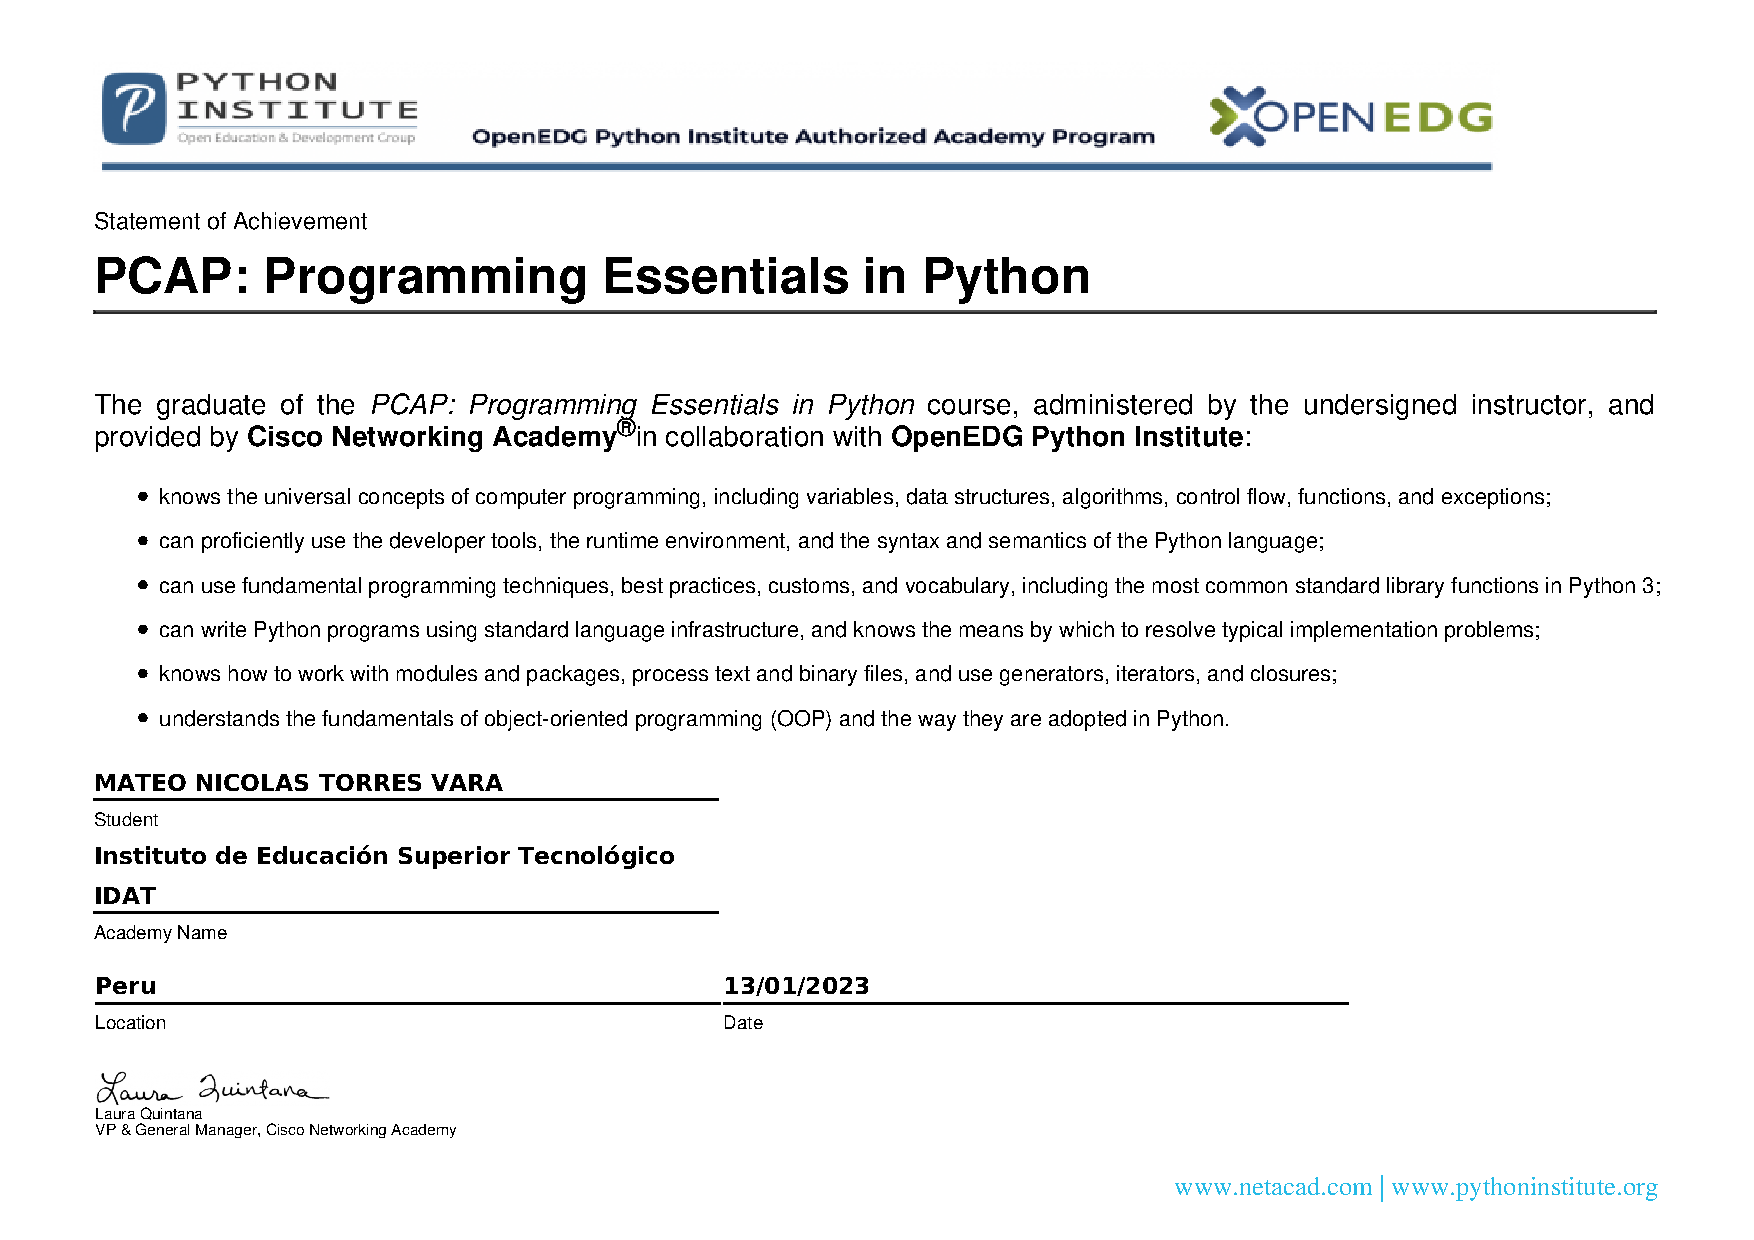
\includepdf[pages=-,landscape,fitpaper=true]{../assets/programming_essentials_in_python.pdf}
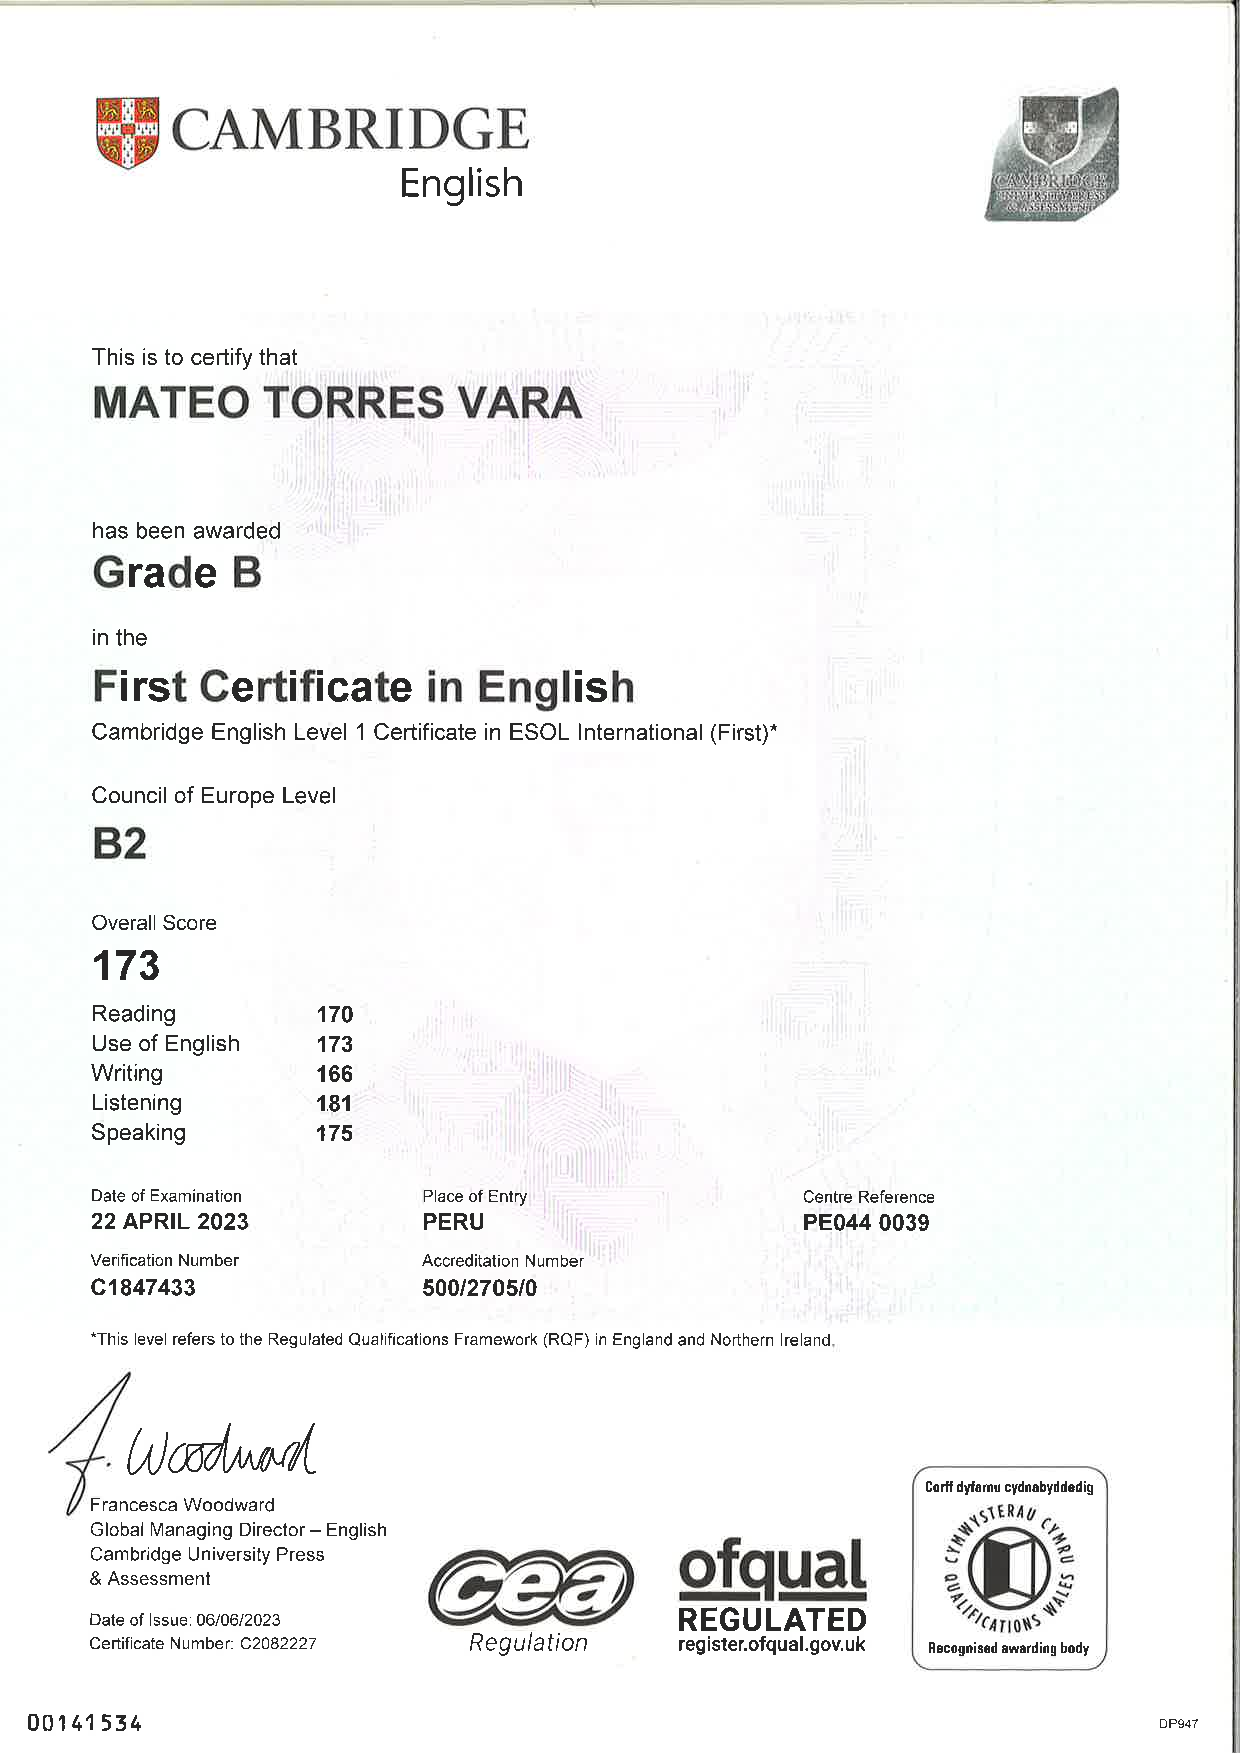
\includepdf[pages=-]{../assets/first_certificate_in_english.pdf}

\end{document}
